\setcounter{section}{4}
\section{TP05 - Regular expressions}
{
\renewcommand{\thesubsubsection}{\thesubsection\alph{subsubsection}}
\subsection{Exercise 1}
\subsubsection{Item a}
\begin{alignat*}{3}
	(\varepsilon + a + aa + aaa)(baaa)^*(\varepsilon + b + ba + baa)
\end{alignat*}
\subsubsection{Item b}
I prefer an $\varepsilon$-NFA because it simplifies the task of recognizing the $\varepsilon$'s of the regular expression when converting from RE to a FA.
\subsubsection{Item c}
\begin{center}
	\begin{tikzpicture}[->,>=stealth',node distance=1.5cm,initial text=$ $,]
		\footnotesize
		\node[state, initial] at (0,-1.8) (0) {$0$};
		\node[state] at (1.2, -0.0) (100) {$100$};
		\node[state] at (1.2, -1.2) (110) {$110$};
		\node[state] at (1.2, -2.4) (120) {$120$};
		\node[state] at (1.2, -3.6) (130) {$130$};

		\node[state] at(2.4, -1.2) (111) {$111$};
		\node[state] at(2.4, -2.4) (121) {$121$}; \node[state] at(3.6, -2.4) (122) {$122$};
		\node[state] at(2.4, -3.6) (131) {$131$}; \node[state] at(3.6, -3.6) (132) {$132$}; \node[state] at(4.8, -3.6) (133) {$133$};
		
		\node[state] at(6.0, -1.8) (2) {$2$};

		
		\node[state] at(7.2, -1.8) (30) {$30$};
		\node[state, below right of=30] (31) {$31$};
		\node[state, below left  of=31] (32) {$32$};
		\node[state, above left  of=32] (33) {$33$};

		\node[state] at(8.4, -1.8) (4) {$4$};

		\node[state] at(9.6, -0.0) (500) {$500$};
		\node[state] at(9.6, -1.2) (510) {$510$}; \node[state] at(10.8, -1.2) (511) {$511$};
		\node[state] at(9.6, -2.4) (520) {$520$}; \node[state] at(10.8, -2.4) (521) {$521$}; \node[state] at(12.0, -2.4) (522) {$522$};
		\node[state] at(9.6, -3.6) (530) {$530$}; \node[state] at(10.8, -3.6) (531) {$531$}; \node[state] at(12.0, -3.6) (532) {$532$}; \node[state] at(13.2, -3.6) (533) {$533$};

		\node[state, accepting] at(14.4, -1.8) (6) {$6$};

		\draw   (0)	edge[left	] node{$\varepsilon$} (100)
				(0)	edge[above	] node{$\varepsilon$} (110)
				(0)	edge[below	] node{$\varepsilon$} (120)
				(0)	edge[left	] node{$\varepsilon$} (130)

				(110) edge[above] node{$a$} (111)
				(120) edge[above] node{$a$} (121) (121) edge[above] node{$a$} (122)
				(130) edge[above] node{$a$} (131) (131) edge[above] node{$a$} (132) (132) edge[above] node{$a$} (133)
				
				(100)	edge[above	] node{$\varepsilon$} (2)
				(111)	edge[above	] node{$\varepsilon$} (2)
				(122)	edge[below	] node{$\varepsilon$} (2)
				(133)	edge[below	] node{$\varepsilon$} (2)

				(2) edge[above] node{$\varepsilon$} (30)

				(30) edge[left	] node{$b$} (31)
				(31) edge[above	] node{$a$} (32)
				(32) edge[right	] node{$a$} (33)
				(33) edge[below	] node{$a$} (30)

				(30) edge[above] node{$\varepsilon$} (4)

				(4)	edge[left	] node{$\varepsilon$} (500)
				(4)	edge[above	] node{$\varepsilon$} (510)
				(4)	edge[below	] node{$\varepsilon$} (520)
				(4)	edge[left	] node{$\varepsilon$} (530)

				(510) edge[above] node{$b$} (511)
				(520) edge[above] node{$b$} (521) (521) edge[above] node{$a$} (522)
				(530) edge[above] node{$b$} (531) (531) edge[above] node{$a$} (532) (532) edge[above] node{$a$} (533)
				
				(500)	edge[above	] node{$\varepsilon$} (6)
				(511)	edge[above	] node{$\varepsilon$} (6)
				(522)	edge[below	] node{$\varepsilon$} (6)
				(533)	edge[below	] node{$\varepsilon$} (6)
				;
	\end{tikzpicture}
\end{center}
This $\varepsilon$-NFA can be trivially simplified into the following $\varepsilon$-DFA.
\begin{center}
	\begin{tikzpicture}[->,>=stealth',node distance=1.5cm,initial text=$ $,]
		\footnotesize
		\node[state, initial] (100) {$100$};
		\node[state, below of=100] (111) {$111$};
		\node[state, below of=111] (122) {$122$};
		
		\node[state, accepting, right of=111] (30) {$30$};
		\node[state, accepting, above of=30] (31) {$31$};
		\node[state, accepting, right of=31] (32) {$32$};
		\node[state, accepting, right of=30] (33) {$33$};

		\draw   (100)	edge[left	] node{$a$} (111)
				(111)	edge[left	] node{$a$} (122)

				(100)	edge[above	] node{$\varepsilon, a$} (30)
				(111)	edge[above	] node{$a$} (30)
				(122)	edge[below	] node{$a$} (30)

				(30) edge[left	] node{$b$} (31)
				(31) edge[above	] node{$a$} (32)
				(32) edge[right	] node{$a$} (33)
				(33) edge[below	] node{$a$} (30)
				;
	\end{tikzpicture}
\end{center}
\subsection{Exercise 2}
\subsubsection{Item a}
\begin{alignat*}{3}
	 (aa)^* (b  (aa)^* ( b + aba ) + ab (aa)^* ( ab + ba ))(aa)^*
\end{alignat*}
\subsubsection{Item b}
Yes it can. Convert the RE to an $\varepsilon$-NFA and then to a DFA $D$. Then, create the DFA $\overline{D}$ describing the complement of $D$ by converting accept states to normal states, and normal states to accept states. Then, convert $\overline{D}$ to a RE.
\pagebreak
\subsection{Exercise 3}
\begin{equation*}
	(0 + 10)^* 11 (0 + 01)^*
\end{equation*}
\subsection{Exercise 4}
\subsubsection{Item a}
Strings with a maximum of one subsequence of consecutive $1$'s, which can only happen at the end.
\subsubsection{Item b}
Strings with at least one subsequence of three consecutive $0$'s.
\subsubsection{Item c}
Strings with no consecutive $1$'s.
\subsection{Exercise 5}
\begin{center} \begin{tabular}{r | l}
	\textbf{Item} & \textbf{Answer} \\ \hline
	a & False \\
	b & True \\
	c & True \\
	d & True
\end{tabular} \end{center}
\subsubsection{Item a}
False, given the string $a$ is accepted by $(a+b)^*$ but not by $(a^* b)^*$.
\subsubsection{Item b}
True, given it can be converted into a DFA, and then into a RE.
\subsubsection{Item c}
True, given $S^*$ is defined by $S \subseteq S^*$ and $v,w \in S^* \implies v+w \in S^*$ means the concatenation of any two strings of $S^*$ was already in $S^*$.
\subsubsection{Item d}
True. The proof is the fact there is an algorithm that transforms a regular expression describing a language with concatenation, union and closure into an $\varepsilon$-DFA, and another algorithm to transform the $\varepsilon$-DFA into a DFA.
\subsection{Exercise 6}
\subsubsection{Item a}
\begin{center}
\begin{tabular}{c c c c}
\begin{tikzpicture}[->,>=stealth',node distance=1.4cm,initial text=$ $,]
	\footnotesize
	\node[state, initial] (1) {$1$};
	\node[state, below of=1] (2) {$2$};
	\node[state, accepting, below of=2] (5) {$5$};
	\node[state, right of=2] (3) {$3$};
	\node[state, right of=3] (4) {$4$};

	\draw   (1)	edge[left	] node{$a$} (2)
			(2)	edge[left	] node{$.$} (5)
			(2)	edge[bend left, above	] node{$\oplus$} (3)
			(3)	edge[bend left, below	] node{$b$} (2)
			(3)	edge[bend left, above	] node{$c$} (4)
			(4)	edge[bend left, below	] node{$\otimes$} (3)
			;
\end{tikzpicture}
&
\begin{tikzpicture}[->,>=stealth',node distance=1.4cm,initial text=$ $,]
	\footnotesize
	\node[state, initial] (1) {$1$};
	\node[state, below of=1] (2) {$2$};
	\node[state, accepting, below of=2] (5) {$5$};
	\node[state, right of=2] (3) {$3$};

	\draw   (1)	edge[left	] node{$a$} (2)
			(2)	edge[left	] node{$.$} (5)
			(2)	edge[bend left, above	] node{$\oplus$} (3)
			(3)	edge[bend left, below	] node{$b$} (2)
			(3)	edge[loop above	] node{$c\otimes$} (3)
			;
\end{tikzpicture}
&
\begin{tikzpicture}[->,>=stealth',node distance=1.4cm,initial text=$ $,]
	\footnotesize
	\node[state, initial] (1) {$1$};
	\node[state, below of=1] (2) {$2$};
	\node[state, accepting, below of=2] (5) {$5$};

	\draw   (1)	edge[left	] node{$a$} (2)
			(2)	edge[loop right	] node{$\oplus(c\otimes)^* b$} (2)
			(2)	edge[left	] node{$.$} (5)
			;
\end{tikzpicture}
&
\begin{tikzpicture}[->,>=stealth',node distance=2.8cm,initial text=$ $,]
	\footnotesize
	\node[state, initial] (1) {$1$};
	\node[state, accepting, below of=1] (5) {$5$};

	\draw   (1)	edge[right	] node{$a(\oplus (c \otimes)^* b)^* .$} (5)
			;
\end{tikzpicture}
\end{tabular}
\end{center}
\begin{equation*}
	a(\oplus (c \otimes )^* b)^* .
\end{equation*}
\subsubsection{Item b}
\begin{equation*}
	a.
\end{equation*}
\subsubsection{Item c}
An infinite number of strings, given the use of the closure operator $^*$.
\pagebreak
\subsection{Exercise 7}
\subsubsection{Item a}
\begin{center}
\begin{minipage}{0.35\textwidth}
\begin{center} \begin{tabular}{r | c c c}
	$\delta_E     $ & $\varepsilon$ & $0        $ & $1        $ \\ \hline
	$\rightarrow A$ & $\{C      \}$ & $\{B    \}$ & $\emptyset$ \\
	$            B$ & $\emptyset  $ & $\emptyset$ & $\{D    \}$ \\
	$            C$ & $\emptyset  $ & $\{C    \}$ & $\{C,D  \}$\\
	$      ^* D$ & $\emptyset  $ & $\emptyset$ & $\emptyset$
\end{tabular} \end{center}
\end{minipage}%
\begin{minipage}{0.25\textwidth}
	\begin{alignat*}{2}
		\varepsilon close(A)&=\{A,C\}\\
		\varepsilon close(B)&=\{B\}\\
		\varepsilon close(C)&=\{C\}\\
		\varepsilon close(D)&=\{D\}\\
	\end{alignat*}
\end{minipage}
\end{center}
\begin{center}
\begin{minipage}[c]{0.44\textwidth}
	\begin{alignat*}{2}
		DFA\,D    &= (Q_D, \Sigma, \delta_D, q_0, F_D)\\
		Q_D      &= \{\{C\},\{A,C\},\{B,C\},\{C,D\}\}\\
		\Sigma   &= \{0,1\}\\
		q_0      &= \{A,C\}\\
		F_D      &= \{\{C,D\}\}\\
		\delta_D &\colon Q_D \times \Sigma \rightarrow Q_D
	\end{alignat*}
\end{minipage}%
\begin{minipage}[c]{0.32\textwidth}
\begin{center} \begin{tabular}{r | c c}
	$\delta_D           $ & $0      $ & $1      $ \\ \hline
	$            \{C  \}$ & $\{C  \}$ & $\{C,D\}$ \\	
	$\rightarrow \{A,C\}$ & $\{B,C\}$ & $\{C,D\}$ \\
	$            \{B,C\}$ & $\{C  \}$ & $\{C,D\}$ \\
	$      ^* \{C,D\}$ & $\{C  \}$ & $\{C,D\}$
\end{tabular} \end{center}
\end{minipage}%
\begin{minipage}[c]{0.24\textwidth}
	\begin{tikzpicture}[->,>=stealth',node distance=2cm,initial text=$ $,]
		\footnotesize
		\node[state, initial] (AC) {$\{A,C\}$};
		\node[state, right of=AC] (BC) {$\{B,C\}$};
		\node[state, accepting, above of=AC] (CD) {$\{C,D\}$};
		\node[state, above of=BC] (C) {$\{C\}$};
	
		\draw   (AC)	edge[above	] node{$0$} (BC)
				(AC)	edge[left	] node{$1$} (CD)

				(BC)	edge[right	] node{$0$} (C)
				(BC)	edge[below	] node{$1$} (CD)

				(CD)	edge[bend left=10,above	] node{$0$} (C)
				(CD)	edge[loop above	] node{$1$} (CD)

				(C)	edge[loop above	] node{$0$} (C)
				(C)	edge[bend left=10, below	] node{$1$} (CD)
				;
	\end{tikzpicture}
\end{minipage}
\end{center}
\subsubsection{Item b}
\begin{center}
	\begin{tabular}{c c c c}
		\begin{tikzpicture}[->,>=stealth',node distance=1.4cm,initial text=$ $,]
			\footnotesize
			\node[state, initial] (A) {$A$};
			\node[state, above of=A] (C) {$C$};
			\node[state, right of=A] (B) {$B$};
			\node[state, accepting, right of=C] (D) {$D$};
		
			\draw   (A)	edge[left	] node{$\varepsilon$} (C)
					(C)	edge[loop above	] node{$0,1$} (C)
					(C)	edge[above	] node{$1$} (D)
					(A)	edge[below	] node{$0$} (B)
					(B)	edge[right	] node{$1$} (D)
					;
		\end{tikzpicture}
		&
		\begin{tikzpicture}[->,>=stealth',node distance=1.4cm,initial text=$ $,]
			\footnotesize
			\node[state, initial] (A) {$A$};
			\node[state, right of=A] (B) {$B$};
			\node[state, accepting, above of=B] (D) {$D$};
		
			\draw   (A)	edge[left	] node{$(0+1)^*$} (D)
					(A)	edge[below	] node{$0$} (B)
					(B)	edge[right	] node{$1$} (D)
					;
		\end{tikzpicture}
		&
		\begin{tikzpicture}[->,>=stealth',node distance=1.9cm,initial text=$ $,]
			\footnotesize
			\node[state, initial] (A) {$A$};
			\node[state, accepting, above right of=A] (D) {$D$};
		
			\draw   (A)	edge[bend left, left	] node{$(0+1)^*$} (D)
					(A)	edge[bend right, below	] node{$01$} (D)
					;
		\end{tikzpicture}
		&
		\begin{tikzpicture}[->,>=stealth',node distance=1.9cm,initial text=$ $,]
			\footnotesize
			\node[state, initial] (A) {$A$};
			\node[state, accepting, above right of=A] (D) {$D$};
		
			\draw   (A)	edge[left	] node{$01+(0+1)^*$} (D)
					;
		\end{tikzpicture}
	\end{tabular}
\end{center}
\begin{equation*}
	01+(0+1)^* 1 = (0+(0+1)^*) 1 = (0+1)^* 1
\end{equation*}
\pagebreak
\subsection{Exercise 8}
\subsubsection{Item a}
\begin{center}
	\begin{tikzpicture}[->,>=stealth',node distance=1.4cm,initial text=$ $,]
		\footnotesize
		\node[state, initial] (0) {$0$};
		\node[state, below of=0] (1) {$1$};
		\node[state, right of=0] (2) {$2$};
		\node[state, accepting, right of=1] (3) {$3$};
	
		\draw   (0)	edge[left	] node{$a$} (1)
				(1)	edge[left	] node{$b$} (2)
				(2)	edge[right	] node{$a$} (3)
				(1)	edge[bend left=10, above	] node{$b$} (3)
				(3)	edge[bend left=10, below	] node{$a$} (1)
				;
	\end{tikzpicture}
\end{center}
$ab$, $abab$, $aba$ are accepted.
\subsubsection{Item b}
Language of strings started in $a$ with no consecutive $b$'s and at most two consecutive $a$'s.
\subsubsection{Item c}
\begin{center} \begin{tabular}{c c c}
\begin{tikzpicture}[->,>=stealth',node distance=1.7cm,initial text=$ $,]
	\footnotesize
	\node[state, initial] (0) {$0$};
	\node[state, below of=0] (1) {$1$};
	\node[state, right of=0] (2) {$2$};
	\node[state, accepting, right of=1] (3) {$3$};

	\draw   (0)	edge[left	] node{$a$} (1)
			(1)	edge[left	] node{$b$} (2)
			(2)	edge[right	] node{$a$} (3)
			(1)	edge[bend left=10, above	] node{$b$} (3)
			(3)	edge[bend left=10, below	] node{$a$} (1)
			;
\end{tikzpicture}
&
\begin{tikzpicture}[->,>=stealth',node distance=1.7cm,initial text=$ $,]
	\footnotesize
	\node[state, initial] (0) {$0$};
	\node[state, below of=0] (1) {$1$};
	\node[state, accepting, right of=1] (3) {$3$};

	\draw   (0)	edge[left	] node{$a$} (1)
			(1)	edge[bend left=10, above	] node{$ba+b$} (3)
			(3)	edge[bend left=10, below	] node{$a$} (1)
			;
\end{tikzpicture}
&
\begin{tikzpicture}[->,>=stealth',node distance=2.3cm,initial text=$ $,]
	\footnotesize
	\node[state, initial] (0) {$0$};
	\node[state, accepting, below right of=0] (3) {$3$};

	\draw   (0)	edge[left	] node{$a(ba+b)$} (3)
			(3) edge[loop right] node{$a(ba+b)$} (3)
			;
\end{tikzpicture}
\end{tabular} \end{center}
\begin{equation*}
	ab(\varepsilon+a)(ab(\varepsilon+a))^*=(ab(\varepsilon+a))^+
\end{equation*}
\subsubsection{Item d}
\begin{center}
\begin{minipage}{0.30\textwidth}
	\begin{center} \begin{tabular}{r | c c}
		$\delta_D           $ & $a        $ & $b        $\\ \hline
		$          \emptyset$ & $\emptyset$ & $\emptyset$\\
		$\rightarrow \{0  \}$ & $\{1    \}$ & $\emptyset$\\
		$            \{1  \}$ & $\emptyset$ & $\{2,3  \}$\\
		$      ^* \{1,3\}$ & $\{1    \}$ & $\{2,3  \}$\\
		$      ^* \{2,3\}$ & $\{1,3  \}$ & $\emptyset$
	\end{tabular} \end{center}
\end{minipage}
\begin{minipage}{0.30\textwidth}
	\begin{center}
		\begin{tikzpicture}[->,>=stealth',node distance=1.7cm,initial text=$ $,]
			\footnotesize
			\node[state, initial] (0) {$\{0\}$};
			\node[state, right of=0] (1) {$\{1\}$};
			\node[state, accepting, right of=1] (23) {$\{2,3\}$};
			\node[state, above of=1] (e) {$\emptyset$};
			\node[state, accepting, below of=23] (13) {$\{1,3\}$};
			
			\draw   (0)		edge[above] node{$a$} (1)
					(1)		edge[above] node{$b$} (23)
					(0)		edge[above] node{$b$} (e)
					(1)		edge[left ] node{$a$} (e)
					(23)	edge[above] node{$b$} (e)
					(13)	edge[below] node{$a$} (1)
					(13)	edge[bend left=10, left ] node{$b$} (23)
					(23)	edge[bend left=10, right] node{$a$} (13)
					;
		\end{tikzpicture}
	\end{center}
\end{minipage}
\end{center}
\subsection{Exercise 9}
\begin{enumerate}
\item Accepts $a$, which is not a valid string per the exercise statement.
\item \label{itm:5_9_2} Enumerates all possible configurations for the blocks of size 3, thus complying with the statement.
\item Does not accept $acb$, although it complies with the exercise statement.
\item Accepts $aaa$, which is not a valid string per the exercise statement.
\end{enumerate}
The correct answer is \ref{itm:5_9_2}.
\pagebreak
\subsection{Exercise 10}
\begin{center} \begin{tabular}{r | c c}
	$\delta_D       $ & $0  $ & $1  $ \\ \hline
	$\rightarrow ^* q_1$ & $q_2$ & $q_3$\\
	$               q_2$ & $q_1$ & $q_3$\\
	$            ^* q_3$ & $q_2$ & $q_1$
\end{tabular} \end{center}
\subsubsection{Item a}
\begin{center} \begin{tabular}{r || c c | c c | c c}
	$k           $ & \multicolumn{2}{c |}{$0$} & \multicolumn{2}{c |}{$1$} & \multicolumn{2}{c}{$2$} \\ \hline
	$R_{11}^{(k)}$ & $\varepsilon$ & $\varepsilon$ & $\varepsilon+\varepsilon\varepsilon^*\varepsilon$& $\varepsilon$ & $\varepsilon+0(\varepsilon+00)^*0$ & $(00)^*$\\
	$R_{12}^{(k)}$ & $0$ & $0$ & $0+\varepsilon\varepsilon^* 0$ & $0$ & $0+0(\varepsilon+00)^*(\varepsilon+00)$ & $0(00)^*$\\
	$R_{13}^{(k)}$ & $1$ & $1$ & $1+\varepsilon\varepsilon^* 1$ & $1$ & $1+0(\varepsilon+00)^*(1+01)$ & $0^*1$\\
	$R_{21}^{(k)}$ & $0$ & $0$ & $0+0\varepsilon^*\varepsilon$ & $0$ & $0+(\varepsilon+00)(\varepsilon+00)^*0$ & $0(00)^*$\\
	$R_{22}^{(k)}$ & $\varepsilon$ & $\varepsilon$ & $\varepsilon+0\varepsilon^* 0$& $\varepsilon+00$ & $\varepsilon+00+(\varepsilon+00)(\varepsilon+00)^*(\varepsilon+00)$ & $(00)^*$\\
	$R_{23}^{(k)}$ & $1$ & $1$ & $1+0\varepsilon^* 1$ & $1+01$ & $1+01+(\varepsilon+00)(\varepsilon+00)^*(1+01)$ & $(00)^*(1+01)$\\
	$R_{31}^{(k)}$ & $1$ & $1$ & $1+1\varepsilon^*\varepsilon$ & $1$ & $1+(0+10)(\varepsilon+00)^*0$ & $(1+00)(00)^*$\\
	$R_{32}^{(k)}$ & $0$ & $0$ & $0+1\varepsilon^* 0$ & $0+10$ & $0+10+(0+10)(\varepsilon+00)^*(\varepsilon+00)$ & $(0+10)(00)^*$\\
	$R_{33}^{(k)}$ & $\varepsilon$ & $\varepsilon$ & $\varepsilon+1\varepsilon^* 1$& $\varepsilon+11$ & $\varepsilon+11+(0+10)(\varepsilon+00)^*(1+01)$ & $\varepsilon+(0+1)0^*1$
\end{tabular} \end{center}
\begin{alignat*}{2}
	R_{13}^{(3)}
	&= 0^*1+0^*1(\varepsilon +(0+1)0^*1)^*(\varepsilon +(0+1)0^*1)\\
	&= 0^*1+0^*1((0+1)0^*1)^*(\varepsilon +(0+1)0^*1)\\
	&= 0^*1((0+1)0^*1)^*(\varepsilon +(0+1)0^*1)\\
	&= 0^*1((0+1)0^*1)^*
\end{alignat*}
\begin{alignat*}{2}
	R_{11}^{(3)}
	&= (00)^* + 0^*1(\varepsilon+(0+1)0^*1)^* (1+00)(00)^* \\
	&= (00)^* + 0^*1((0+1)0^*1)^* (1+00)(00)^* 
\end{alignat*}
\begin{alignat*}{2}
	R_{11}^{(3)}+R_{13}^{(3)}
	&= 0^*1((0+1)0^*1)^* + (00)^* + 0^*1((0+1)0^*1)^* (1+00)(00)^* \\
	&= 0^*1((0+1)0^*1)^* + 0^*1((0+1)0^*1)^* (1+00)(00)^* + (00)^* \\
	&= 0^*1((0+1)0^*1)^*(\varepsilon + (1+00)(00)^*) + (00)^* \\
	&= 0^*1((0+1)0^*1)^*(\varepsilon + 1(00)^*+(00)^+) + (00)^* \\
	&= 0^*1((0+1)0^*1)^*(1(00)^*+(00)^*) + (00)^* \\
	&= 0^*1((0+1)0^*1)^*(\varepsilon + 1)(00)^* + (00)^* \\
	&= (00)^*  + 0^*1((0+1)0^*1)^*(\varepsilon + 1)(00)^*
\end{alignat*}
\subsubsection{Item b}
\begin{center}
\begin{minipage}{0.30\textwidth}
	\begin{center} 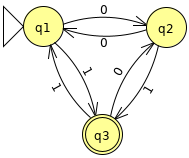
\includegraphics[scale=0.5]{TP05_10_b_1} \end{center}
	\begin{center} 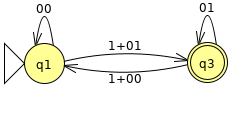
\includegraphics[scale=0.5]{TP05_10_b_2} \end{center}
\end{minipage}%
\begin{minipage}{0.60\textwidth}
	\begin{alignat*}{2}
	 	 & (00)^*(1+01)           &&(01 + (1+00)(00)^*(1+01))^*\\
		=& (00)^*(\varepsilon+0)1 &&(01 + 1(00)^*(1+01)+00(00)^*(1+01))^*\\
		=& 0^*1                   &&(01 + 1(00)^*(\varepsilon+0)1+00(00)^*(1+01))^*\\
		=& 0^*1                   &&(01 + 10^*1+00(00)^*(1+01))^*\\
		=& 0^*1                   &&(01 + 10^*1+00(00)^*(\varepsilon+0)1)^*\\
		=& 0^*1                   &&(01 + 10^*1+000^*1)^*\\
		=& 0^*1                   &&(01 +000^*1 + 10^*1)^*\\
		=& 0^*1                   &&(0(\varepsilon +00^*)1 + 10^*1)^*\\
		=& 0^*1                   &&(0(\varepsilon +0^+)1 + 10^*1)^*\\
		=& 0^*1                   &&(00^*1 + 10^*1)^*\\
		=& 0^*1                   &&((0+1)0^*1)^*
	\end{alignat*}
\end{minipage}
\end{center}
\begin{center}
\begin{minipage}{0.30\textwidth}
	\begin{center} 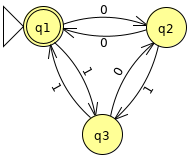
\includegraphics[scale=0.5,trim={0  7mm 0 0}]{TP05_10_b_1_2} \end{center}
	\begin{center} 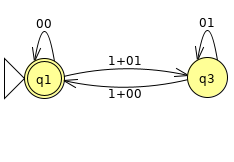
\includegraphics[scale=0.5,trim={0 20mm 0 0}]{TP05_10_b_2_2} \end{center}
	\begin{center} 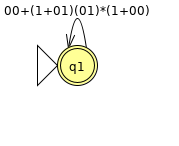
\includegraphics[scale=0.5,trim={0 20mm 0 0}]{TP05_10_b_3_2} \end{center}
\end{minipage}%
\begin{minipage}{0.60\textwidth}
	\begin{alignat*}{2}
	 	 & (00+(1+01)(01)^*(1+00))^*\\
		=& (00+(1+01)01^*(0+1))^* \\
		=& (00+(\varepsilon+0)101^*(0+1))^*
	\end{alignat*}
\end{minipage}
\end{center}
\begin{alignat*}{2}
	0^*1((0+1)0^*1)^* + (00+(\varepsilon+0)101^*(0+1))^*
\end{alignat*}
\subsection{Exercise 11}
The correct answer is NE.
\begin{center} 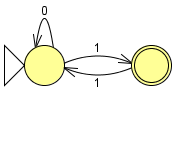
\includegraphics[scale=0.5]{TP05_11} \end{center}
}
